\documentclass{article}

% if you need to pass options to natbib, use, e.g.:
\PassOptionsToPackage{numbers, compress}{natbib}
% before loading nips_2017
%
% to avoid loading the natbib package, add option nonatbib:
% \usepackage[nonatbib]{nips_2017}

\usepackage{nips_2018}

% to compile a camera-ready version, add the [final] option, e.g.:
% \usepackage[final]{nips_2017}

\usepackage[utf8]{inputenc} % allow utf-8 input
\usepackage[T1]{fontenc}    % use 8-bit T1 fonts
\usepackage{hyperref}       % hyperlinks
\usepackage{url}            % simple URL typesetting
\usepackage{booktabs}       % professional-quality tables
\usepackage{amsfonts}       % blackboard math symbols
\usepackage{nicefrac}       % compact symbols for 1/2, etc.
\usepackage{microtype}      % microtypography

\usepackage{hyperref}

\usepackage{amssymb}
\usepackage{amsmath}

% For citations
\usepackage{natbib}

% For figures
\usepackage{graphicx} % more modern
\usepackage{wrapfig}
%\usepackage{epsfig} % less modern
\usepackage{subfigure} 
\usepackage{multirow}
\usepackage{adjustbox}

\usepackage{listings}
\usepackage{textcomp}

% For assumptions
\usepackage{amsthm,amssymb,amsopn}
\newtheorem{assumption}{Assumption}
\newtheorem{define}{Definition}
\newtheorem{thm}{Theorem}
\newtheorem{lem}{Lemma}
\newtheorem{coro}{Corollary}
\newtheorem{condition}{Condition}

% For algorithms
\usepackage{algorithm}
\usepackage{algorithmic}
\renewcommand{\algorithmicrequire}{\textbf{Input:}}
\renewcommand{\algorithmicensure}{\textbf{Output:}}
\makeatletter
\makeatletter
\newcommand*{\da@rightarrow}{\mathchar"0\hexnumber@\symAMSa 4B }
\newcommand*{\da@leftarrow}{\mathchar"0\hexnumber@\symAMSa 4C }
\newcommand*{\xdashrightarrow}[2][]{%
  \mathrel{%
    \mathpalette{\da@xarrow{#1}{#2}{}\da@rightarrow{\,}{}}{}%
  }%
}
\newcommand{\xdashleftarrow}[2][]{%
  \mathrel{%
    \mathpalette{\da@xarrow{#1}{#2}\da@leftarrow{}{}{\,}}{}%
  }%
}
\newcommand*{\da@xarrow}[7]{%
  % #1: below
  % #2: above
  % #3: arrow left
  % #4: arrow right
  % #5: space left 
  % #6: space right
  % #7: math style 
  \sbox0{$\ifx#7\scriptstyle\scriptscriptstyle\else\scriptstyle\fi#5#1#6\m@th$}%
  \sbox2{$\ifx#7\scriptstyle\scriptscriptstyle\else\scriptstyle\fi#5#2#6\m@th$}%
  \sbox4{$#7\dabar@\m@th$}%
  \dimen@=\wd0 %
  \ifdim\wd2 >\dimen@
    \dimen@=\wd2 %   
  \fi
  \count@=2 %
  \def\da@bars{\dabar@\dabar@}%
  \@whiledim\count@\wd4<\dimen@\do{%
    \advance\count@\@ne
    \expandafter\def\expandafter\da@bars\expandafter{%
      \da@bars
      \dabar@ 
    }%
  }%  
  \mathrel{#3}%
  \mathrel{%   
    \mathop{\da@bars}\limits
    \ifx\\#1\\%
    \else
      _{\copy0}%
    \fi
    \ifx\\#2\\%
    \else
      ^{\copy2}%
    \fi
  }%   
  \mathrel{#4}%
}
\makeatother

% for todos
\usepackage{xargs}                      % Use more than one optional parameter in a new commands
\usepackage[pdftex,dvipsnames]{xcolor}
%todos -- remove at end
\usepackage[colorinlistoftodos,prependcaption,textsize=tiny]{todonotes}
\newcommand{\unsure}[2][1=]{\todo[linecolor=red,backgroundcolor=red!25,bordercolor=red,#1]{#2}}
\newcommand{\change}[2][1=]{\todo[linecolor=blue,backgroundcolor=blue!25,bordercolor=blue,#1]{#2}}
\newcommand{\info}[2][1=]{\todo[linecolor=OliveGreen,backgroundcolor=OliveGreen!25,bordercolor=OliveGreen,#1]{#2}}
\newcommand{\improvement}[2][1=]{\todo[linecolor=Plum,backgroundcolor=Plum!25,bordercolor=Plum,#1]{#2}}



\title{Predicting Electron Paths}

% The \author macro works with any number of authors. There are two
% commands used to separate the names and addresses of multiple
% authors: \And and \AND.
%
% Using \And between authors leaves it to LaTeX to determine where to
% break the lines. Using \AND forces a line break at that point. So,
% if LaTeX puts 3 of 4 authors names on the first line, and the last
% on the second line, try using \AND instead of \And before the third
% author name.

\author{
  David S.~Hippocampus\thanks{Use footnote for providing further
    information about author (webpage, alternative
    address)---\emph{not} for acknowledging funding agencies.} \\
  Department of Computer Science\\
  Cranberry-Lemon University\\
  Pittsburgh, PA 15213 \\
  \texttt{hippo@cs.cranberry-lemon.edu} \\
  %% examples of more authors
  %% \And
  %% Coauthor \\
  %% Affiliation \\
  %% Address \\
  %% \texttt{email} \\
  %% \AND
  %% Coauthor \\
  %% Affiliation \\
  %% Address \\
  %% \texttt{email} \\
  %% \And
  %% Coauthor \\
  %% Affiliation \\
  %% Address \\
  %% \texttt{email} \\
  %% \And
  %% Coauthor \\
  %% Affiliation \\
  %% Address \\
  %% \texttt{email} \\
}

\newcommand{\xb}{\mathbf{x}}
\newcommand{\Xc}{\mathcal{X}}
\newcommand{\Zc}{{\mathcal{Z}}}
\newcommand{\Mc}{{\mathcal{M}}}
\newcommand{\Bc}{{\mathcal{B}}}
\newcommand{\Ac}{{\mathcal{A}}}
\newcommand{\Pc}{{\mathcal{P}}}
\newcommand{\bb}{{\mathbf{b}}}
\newcommand{\ab}{{\mathbf{a}}}
\newcommand{\mb}{{\mathbf{m}}}
\newcommand{\Mb}{{\mathbf{M}}}
\newcommand{\Pb}{{\mathbf{P}}}
\newcommand{\Hb}{{\mathbf{H}}}
\newcommand{\Ab}{{\mathbf{A}}}
\newcommand{\Rc}{{\mathcal{R}}}
\newcommand{\delb}{{\boldmath{\delta}}}


%
\newcommand{\nodeEmbeddings}[1]{\Hb_{#1}}
\newcommand{\graphEmbeddings}{\mathbf{h_g}}
%\newcommand{\graph}{\mathcal{G}}



\newcommand{\actionLogits}{\textbf{s}} % for nodes

% The model definitions
\newcommand{\electronPath}{\Pc}
\newcommand{\moleculeSet}{\Mc}
\newcommand{\initialAndReactants}{\Mc_0, \Mc_r}

\newcommand{\contextVect}{\bm{c}}
% Then the modules!
\newcommand{\fEmbed}{g_{\Ac}} % for nodes
\newcommand{\fEmbedGraphs}{r} % for nodes


\newcommand{\fAdd}{f_{\textrm{add}}}
\newcommand{\fRemove}{f_{\textrm{remove}}}
\newcommand{\fInitial}{f_{\textrm{initial}}}
\newcommand{\fStop}{f_{\textrm{stop}}}
\newcommand{\fReagEmbed}{f_{\textrm{reagent}}}
\newcommand{\fModules}{\fEmbed, \fAdd, \fRemove, \fInitial,\fStop, \fReagEmbed}
\newcommand{\fui}{f_i}
\newcommand{\fuj}{f_j}
\newcommand{\fuk}{f_k}
\newcommand{\fum}{f_m}

\newcommand{\actionProb}[2][]{ p(a_{#2} \mid \moleculeSet_{\electronPath_{0:#2-1}^{#1}}, a^{#1}_{#2-1}, #2)}
\newcommand{\continueProb}[2]{p(s_{#1}' \mid \moleculeSet_{#2}) }

\begin{document}
% \nipsfinalcopy is no longer used

\maketitle

\begin{abstract}
The vast majority of chemical reactions can be described as the movement of pairs of electrons through a set of reactant molecules. 
As such, reactions are often described using `arrow-pushing' diagrams which show this movement as a sequence of arrows. We propose to learn this sequence directly. 
Instead of predicting product molecules directly from reactant molecules in one-shot, learning a model of electron movement has the benefits of 
(a) being easy for chemists to interpret, 
(b) being able to incorporate the constraints of chemistry such as balanced atom counts each side, and 
(c) naturally encoding the sparsity of chemical reactions, which usually involve only a small number of atoms in the reactants.
Furthermore, we show that the model recovers basic knowledge of chemistry without being explicitly trained to do so.
% also it means the sides balance
\end{abstract}




\section{Background}
In this section we describe the types of reactions we consider in this paper, and how it relates to previous work on reaction prediction. We then describe recent related work on deep graph models that inspire our model in the following section.

\paragraph{Chemical reactions.}
Molecules consist of a set of atoms that are arranged into a structure by a set of bonds. As such, molecules can be depicted as a graph structure, where each node is an atom and each edge is a bond, as shown in Figure (note the convention that vertices which do not explicitly specify the atom name are assumed to be carbon C atoms). 

In reality, the structure of a molecule is due to how electrons on each atom are interacting with each other. Each single bond represents the fact that two electrons are shared between the atoms that the bond connects\footnote{The vast majority of bonds in molecules are like this (so-called \emph{covalent} bonds), although our model also accommodates ionic bonds (in which one atom completely borrows the electrons of another atom and the atoms become charged ions.}.

%Molecules are broken and built via reactions. 
Just as electrons describe the current structure of molecules, they also describe how molecules react with other molecules to produce new ones. All chemical reactions involve the movement of electrons along paths of atoms in a set of reactant molecules. This movement causes the formation and breaking of chemical bonds that changes the reactants into a new set of product molecules.\footnote{This movement happens because it allows the set of molecules to move to a lower (and thus more favorable) energy state.} In this work, we will consider reactions that satisfy the following assumptions:
% \begin{enumerate}
% \item are single-step, so-called \emph{elementary} reactions.
% \item involve a pair of electrons, so-called \emph{heterolytic} reactions.
% \item either start with electrons on single atom, or with the electrons in an existing bond.
% \end{enumerate}
\begin{assumption}
Reactions are single-step, so-called \emph{elementary} reactions.
\label{assume:elem}
\end{assumption}

\begin{assumption}
Reactions involve pairs of electrons moving, so-called \emph{heterolytic} reactions.
\label{assume:het}
\end{assumption}

\begin{assumption}
Reactions either start with electrons on single atom (called \emph{free electrons}), or with the electrons in an existing bond.
\label{assume:atom_bond}
\end{assumption}

These sorts of reactions describes the vast majority of \emph{organic reactions} (i.e., reactions involving Carbon atoms) that have a large number of applications from drug design to the invention of new materials\footnote{Organic reactions that do not satisfy these assumptions are homolytic reactions, and concerted reactions.}. For this reason organic reactions has been the focus of recent work in reaction prediction in machine learning \cite{jin2017predicting,schwaller2017found}. Note that reactions which are multi-step can be decomposed into multiple single-step reactions in order to satisfy Assumption~\ref{assume:elem}.


\paragraph{Reactions as single electron paths.}
If reactions satisfy the above assumptions, then a chemical reaction is the result of pairs of electrons moving in a \emph{single path} through the reactant atoms. Further, this electron path will alternately remove existing bonds in molecules, and form new ones. We show this alternating structure in two example single-path reactions in Figure~\ref{fig:example}. In Figure~\ref{fig:example}(a) the reaction starts with the electrons in a bond, and in Figure~\ref{fig:example}(b) the reaction starts with the electrons in an atom. 

There are a number of benefits of predicting electron paths over predicting the outcomes of reactions directly (as in previous work \cite{jin2017predicting,schwaller2017found}):
\begin{itemize}
\item \textbf{Easy to interpret}: If the model makes a mistake, it is easy to see where it goes wrong by comparing the steps of the path with the correct steps.
\item \textbf{Sparse}: Reactions often only affect between 3 and 7 atoms out of anywhere from 10-50 reactant atoms. Modeling the reaction as a path allows us to exploit this sparsity.
\item \textbf{Chemical constraints}: Learning a path allows us to easily incorporate chemical constraints, such as the alternating removal and addition of bonds, among others.
\end{itemize}

\paragraph{Formal notation.}
Below is the formal notation we will use to build a model that describes reactions as electron paths:
\begin{itemize}
\item A maximum number of path timesteps $T$.
\item An initial set of reactant molecules $\Mc_0$, this is a set of molecular graphs with vertices called atoms $\Ac$ and edges called bonds $\Bc$. %We also assume we have a continuous representation of the set of molecules: $\mb_1$, of atoms $\ab$, and bonds $\bb$.
\item A final set of product molecules $\Mc_T$. %, and its continuous representation: $\mb_T$. 
Note, that if we believe it requires less than $T$ steps to go from the reactants to the products we assume we can perform a 'null' step in which the electrons do not move, thus the molecules do not change.
\item A reaction is just a sequence of electron movements from atom to atom. Formally, we write an electron path as an ordering of single atoms $\Pc = (a_0, a_1, \ldots, a_{T-1})$. %, with continuous representation $\Pb = [\ab_1, \ldots, \ab_{T-1}]$.
\end{itemize}


\begin{figure*}
\centering
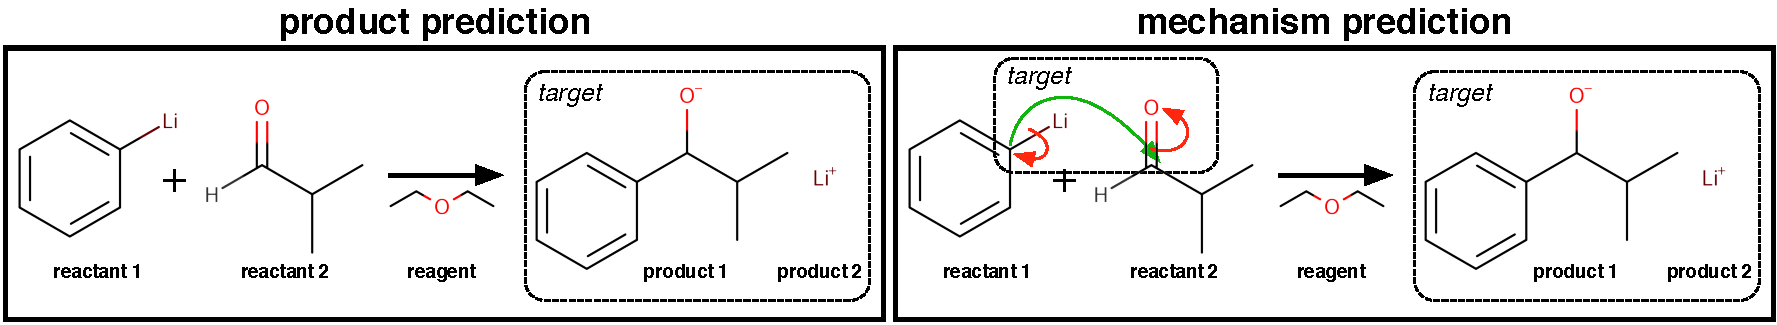
\includegraphics[width=\textwidth]{reaction_diagram}
\caption{reactions}
\end{figure*}

\begin{figure*}
\centering
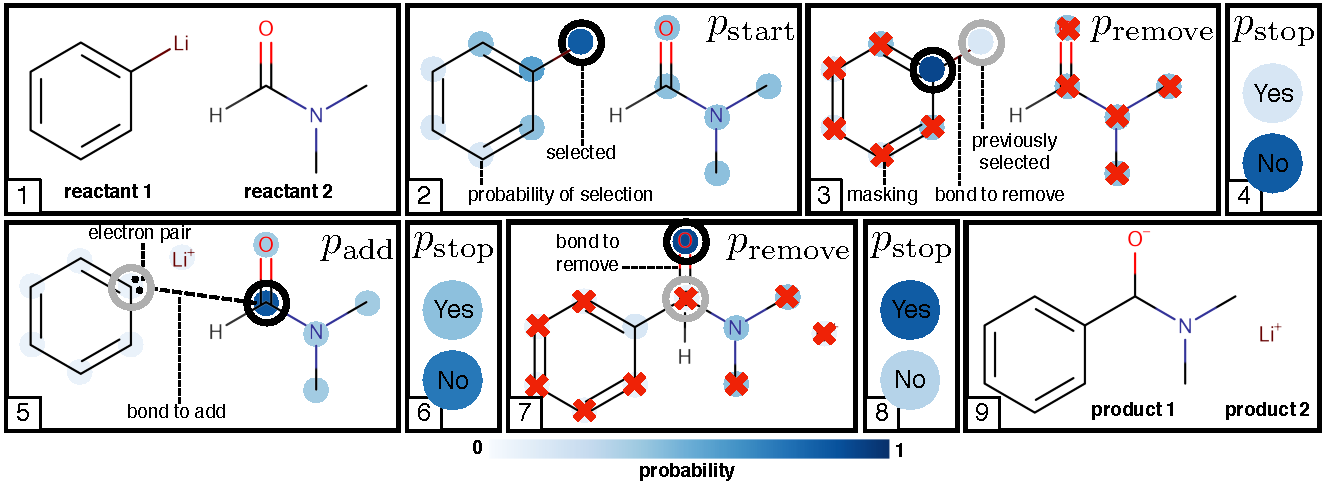
\includegraphics[width=\textwidth]{reaction_model_blue}
\caption{model}
\end{figure*}


\begin{figure*}
\centering
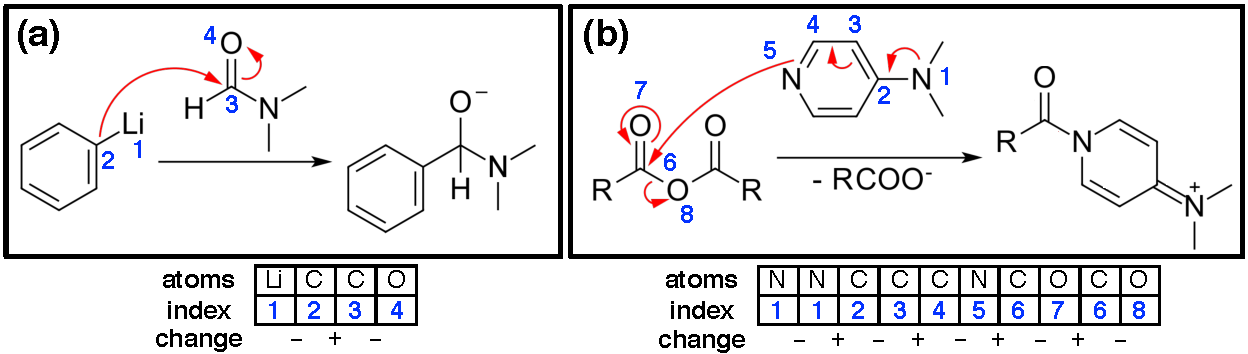
\includegraphics[width=\textwidth]{rxn_example}
\vspace{-3ex}
\caption{Two example reactions and their electron paths. In reaction (a), the reaction starts from an existing bond between Lithium (atom 1) and Carbon (atom 2). In reaction (b) the reaction starts from a lone-pair of electrons on Nitrogen (atom 1), which we represent formally as a bond with itself.}
\label{fig:example}
\end{figure*}

% KEY: separate assumptions from data processing
% !TEX root =  ../main.tex

\section{Model}



\begin{figure*}
\centering
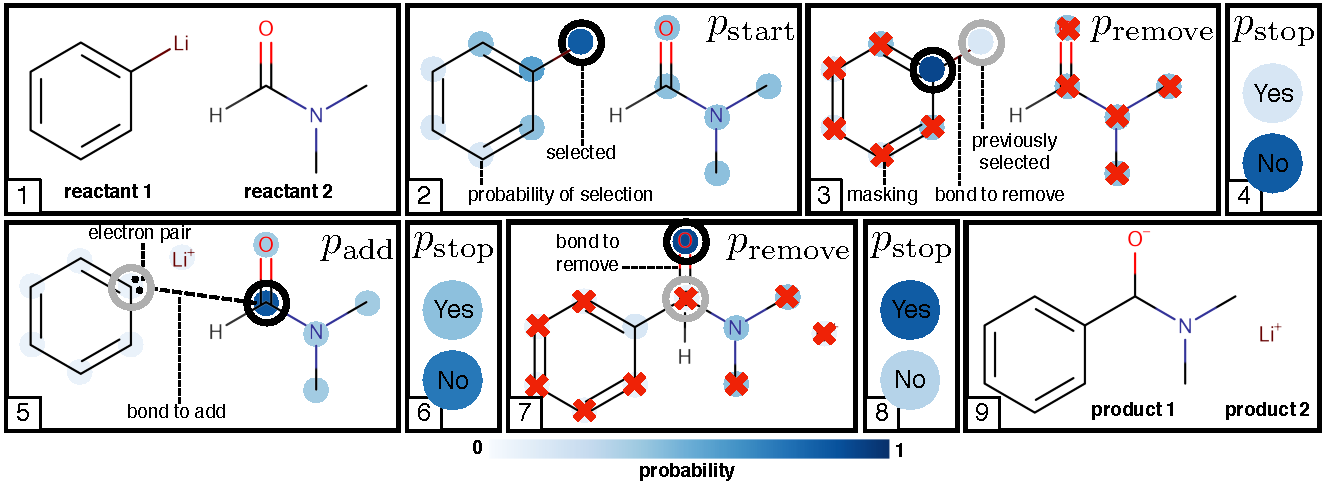
\includegraphics[width=\textwidth]{reaction_model_blue}
\caption{A visualization of the actions taken by the model to sequentially perform a simple reaction.}
\label{fig:reaction_model}
\end{figure*}



In this section we define a probabilistic model that describes the flow of movement of electrons that define an elementary heterolytic reaction.
We represent a set of molecules as a set of graphs $\moleculeSet$, with atoms $\Ac$ as vertices and bonds $\Bc$ as edges;
each connected component of the graph defines an individual molecule.
We can associate an ordering over all the atoms in all the molecules in the set using an {\em atom map} number,
an integer label assigned to each non-hydrogen atom in both the reactants and the products which 
both permits easy matching between atoms before and after the reaction, and
%\footnote{In the USPTO dataset, all reactions have been ``atom mapped'', which means that integer labels have been assigned to each non-hydrogen atom in both the reactants and the products.}. 
gives us a consistent way to index particular atoms.
Each atom $v \in \Ac$ includes a set of features, such as its atom type (e.g. carbon, oxygen, \dots); the full list of input atom features can be found in Table 1 of the supplementary material.
Input molecules into the model are first put in a Kekul\'e form, a process which makes explicit the location of single and double bonds in aromatic structures;
each bond $b \in \Bc$ is either a single, double, or triple bond.


Given an initial set of reactant molecules $\moleculeSet_0$ and a set of reagent molecules $\moleculeSet_r$, 
our model defines a conditional distribution over a sequence of atoms $\electronPath_{0:T} = (a_0, a_1, \ldots, a_T)$,
which fully characterizes the electron path.
\improvement[]{maybe instead $\electronPath$ goes up to $T-1$ and $\moleculeSet$ goes up to $T$? then both are length $T$}
This electron path in turn deterministically defines both a final product $\moleculeSet_{T+1}$, 
denoting the outcome of the reaction,
as well as a sequence of intermediate products $\moleculeSet_t$, for $t = 1,\dots,T$,
which correspond to the state of the graph after the first $t$ steps in the subsequence $\electronPath_{0:t} = (a_0, \dots, a_t)$ are applied to the initial $\moleculeSet_0$.


We propose to learn a parameterized distribution $p_\theta( \electronPath_{0:T} \mid \moleculeSet_0, \moleculeSet_r)$ over electron movements. 
We begin by describing the generative process %(i.e., the forward pass) 
of $p_\theta$, and then describe how to train the model parameters.


\subsection{Generative process}

The joint probability of an electron path can be factorized into a product of distributions
defining the probability $p(a_0 \mid \initialAndReactants)$ of the initial state $a_0$ given the reactants and reagents, 
the conditional probability $p(a_t \mid a_{t-1}, \moleculeSet_t, t)$ \todo[]{maybe somehow refer to "bond type" instead of $t$?} of next state $a_t$ given the intermediate products $\moleculeSet_t$ for $t > 0$,
and the probability $p(s_t \mid \moleculeSet_t)$ that the reaction terminates with final product $\moleculeSet_{t}$.

%The distribution over electron paths can be factorized as follows:
%%\begin{align}
%%p_\theta(\electronPath \mid \moleculeSet_0) = p_\theta(s_{0}' \mid \moleculeSet_0) p_\theta(a_{0} \mid \moleculeSet_0) \prod_{t=1}^{T-1} \left( p_\theta(a_{t} \mid a_{t-1}, \Mc_{t-1} ) p_\theta(s_{0}' \mid \moleculeSet_0) \right) p_\theta(a_{T} \mid a_{T}, \Mc_{T-1} ) p_\theta(s_{T} \mid \moleculeSet_T) \nonumber
%%\end{align}
%
%\begin{align*}
%p(\electronPath_{0:T} \mid \initialAndReactants) = &
% \quad 
% p(s_0' \mid \initialAndReactants)
% p(a_0 \mid \initialAndReactants)
% \prod_{t=1}^{T} \Big[ 
% 	p(s_t' \mid \initialAndReactants, \electronPath_{0:t-1})
% 	p(a_t \mid \initialAndReactants, \electronPath_{0:t-1} ) 
% \Big] \\
% & \times p(s_{T+1} \mid  \initialAndReactants, \electronPath_{0:T} )
%\end{align*}

%\improvement[]{this part a bit messy}
%Where $p(s_{t})$ is the probability of stopping the path before picking the $t^{\text{th}}$ action, $p(s_{t}')$ of continuing.


In practice we assume that the probability of an action depends only on (i) the intermediate molecule formed by the action path up to that point, (ii) the previous action taken (indicating where the free pair of electrons are) and (iii) the point of time through the path, indicating whether we are on an add or remove bond step. 
We further make the simplifying assumption that the stop probability and the actions after $a_0$ do not depend on the reagents. This leads to a parameterized model with dependency structure:
\begin{align}
\label{eq:jointprob}
p_\theta(\electronPath_{0:T} \mid \moleculeSet_0, \moleculeSet_r) 
&=
	p_\theta(s'_0 \mid \moleculeSet_0)
	p_\theta(a_0 \mid \moleculeSet_0, \moleculeSet_r)\\ \nonumber &\quad \times
	\left[\prod_{t=1}^{T}
		p_\theta(s_{t}' \mid \moleculeSet_{t})
		p_\theta(a_t \mid \moleculeSet_{t}, a_{t-1}, t)
	\right]
	p_\theta(s_{T+1} \mid \moleculeSet_{T+1})
	,
\end{align}
where we have defined $p(s'_t \mid \moleculeSet_t) \equiv 1 - p(s_t \mid \moleculeSet_t)$ to be the probability of {\em continuing} a reaction given the current molecule set $\moleculeSet_t$.
%
%
%%% THIS IS THE PREVIOUS VERSION:
%\begin{align*}
%p_\theta(\electronPath_{0:T} \mid \moleculeSet_0, \moleculeSet_r) = &
% \quad \continueProb{0}{0}
%       p(a_0 \mid \moleculeSet_0, \moleculeSet_r)
%       p(a_1 \mid \moleculeSet_0, a_0) \\
%       & \times \prod_{t=2}^{T} \Big[
%              \continueProb{t}{\electronPath_{0:t-1}}
%              \actionProb{t}
%       \Big] \\
%       & \times p(s_{T+1} \mid \moleculeSet_{\electronPath_{0:T}})
%\end{align*}
%
Note that you cannot stop after one action, as you have to pick up a complete electron pair;
however, it is possible to stop prior to selecting a first atom $a_0$, indicating that no reaction would take place.
Given any particular selected atom $a_t$ which extends the reaction path, we can deterministically update the previous molecular graph $\moleculeSet_{t}$ to produce the next set of (intermediate) products $\moleculeSet_{t+1}$.

If the three reaction assumptions stated in the previous section hold, then, as stated earlier, there are two types of electron movements that alternate: 
(1) movement that \emph{removes an existing bond}, and 
(2) movement that \emph{adds a new bond}. 
We can generalize assumption 3 by defining that atoms with free electrons have a self-bond. 
Thus, all reactions start by first selecting an atom, removing a bond (between two different atoms, or a self-bond), and then alternately adding and removing bond;
we can determine whether a particular step is an add step or remove step by inspecting $t$.
Note that $\moleculeSet_1 = \moleculeSet_0$, as the initial action of selecting $a_0$ does not remove or form any bonds\todo{maybe put this somewhere else}.

Each of the conditional probabilities in Eq.~\eqref{eq:jointprob} is parameterized by a neural network:
for each stage the network takes the current intermediate product graph, 
along with the previous action and the reagents if relevant, 
to compute a probability distribution over next possible actions (i.e., selecting a particular atom, or stopping).
These structure of these networks will be described in the following section and more detailed information on the architectures is given in the supplementary material.

Figure~\ref{fig:reaction_model} shows a simple example reaction, which demonstrates all the critical features of the model.
The first subfigure shows two reactants, which we assume will react (i.e.\ $s_0' = 1$).
Subsequent subfigures show the network picking an initial atom to begin the electron path,
and then iteratively selecting atoms for removing and adding bonds, potentially stopping after each action.
Masking at each add and remove step can reduce the total number of possibilities: 
for example, it is not possible to remove a bond which does not exist in the graph $\moleculeSet_t$.
\todo[]{walk through figure. do we want to that HERE, or in the caption? or elsewhere?}

\subsection{Computing atom and molecule features}


We are left now with defining the functional form of our conditional distributions for continuing $p_\theta(s'_t \mid \moleculeSet_t)$, picking the initial action $p_\theta(a_0 \mid \initialAndReactants)$, and picking subsequent actions $p_\theta(a_t \mid a_{t-1}, \moleculeSet_t, t)$.
However, before describing these modules we need to describe how we compute node embeddings and graph embeddings as these  are  essential to each.
Full architectural details (e.g.\ number of layers and hidden units) are deferred to the supplemental material.

Node embeddings are representations of all the atoms (vertices) in all the molecules present in $\moleculeSet_t$.
 We denote them by the matrix $\nodeEmbeddings{\moleculeSet_t} \subseteq \Rc^{|\Ac|\times d}$.
Each row contains a $d$-dimensional embedding of an atom (vertex).
A natural ordering for the rows are  the corresponding atoms' atom-mapped numbers.
We define the function $\fEmbed$ to take in a set of graphs representing each molecule and compute these node embeddings.
In general $\fEmbed$ could be any deep graph model that uses the graph structure of $\Mc_t$ to get graph-isomorphic node features, usually via message-passing techniques \citep{gilmer2017neural};
we choose to use gated graph neural network (GGNN) message functions \citep{li2016gated}.

It is also useful to be able to calculate graph embeddings $\graphEmbeddings$, which are vectors that represent groups of nodes belonging to one or more graphs; i.e.\ an entire molecule or set of molecules.
 We define the function that takes node features belonging to one or more graphs, and calculates their graph embedding by $\fEmbedGraphs$.
These are similar to the readout functions used for regressing on graphs detailed in \citep[Eq. 3]{gilmer2017neural} and the graph embeddings described in \citet[\S B.1]{li2018learning}. \todo[]{check ref the correct parts of these other papers.}
Specifically, $\fEmbedGraphs$ consists of three functions, $\fui$, $\fuj$ and $\fuk$, which could be any MLP but in practice we find that linear functions suffice. % use linear layers for.
There are two stages:
In stage (i), similar to \citet[\S B.1]{li2018learning} we form an embedding of one or more graphs (with vertices $\Ac'$), by performing a gated sum over the node features
\todo{BP: i added $\fuk$ to this equation, so it was all together --- hope this does not cause notational problems elsewhere}
\begin{align}
	\graphEmbeddings = \fuk\big(\sum_{v \in \Ac'} \left[ \mbox{sigmoid}(\fui(\Hb_{\Ac,v})) \cdot \fuj(\Hb_{\Ac,v}) \right]\big).
\end{align}

In this manner the function $\fui$ is used to decide how much that node should contribute towards the embedding,
 and $\fuj$ projects the node embedding up to a higher dimensional space; following \citet[\S B.1]{li2018learning}, we choose to be double the dimension of the node features.
Having formed this embedding of the graphs, we project this down to a lower dimensional space, which is done by the function $\fuk$. 
%Again we use a single linear layer for this function. % already said this above


\subsection{Computing our probabilities over actions}

Having described how we compute node and graph embeddings we are now ready to describe each of our action modules. We start with $p_\theta(s'_t \mid \moleculeSet_t)$, which is the probability of continuing given the set of intermediate products at time $t$. This probability is computed as a graph embedding down to one dimension followed by a sigmoid function: $p_\theta(s'_t \mid \moleculeSet_t) = \sigma(\fEmbedGraphs_{\textrm{stop}}(\nodeEmbeddings{\moleculeSet_t}))$.


This leaves us with describing the form of the initial action, $p_\theta(a_0 \mid \initialAndReactants)$, and picking subsequent actions, $p_\theta(a_t \mid a_{t-1} \moleculeSet_t, t)$, modules.
 The second of these can be broken down into two parameterized functions
$p_\theta^\textrm{remove}(a_t \mid a_{t-1}, \moleculeSet_t)$ for the remove bond step, taken when $t$ is odd, and $p_\theta^\textrm{add}(a_t \mid \moleculeSet_t, a_{t-1})$ for the add bond step, taken when $t$ is even. 
 Each of these three parameterized conditional probability distributions for the {\em initial}, {\em add} and {\em remove} steps have similar forms, and produce a probability vectors over actions as their output. 
 
 Each of these modules start by computing  a single value for each node, so for the initial step we have 
 $\actionLogits_{\textrm{initial}, v} = \fum^\textrm{intial}(\nodeEmbeddings{\moleculeSet_t,v}, \contextVect)$ where $\fum$ is a NN and $\contextVect$ is a context vector. The expressions are similar for the add and remove modules, however with different NNs used for the respective $\fum$ functions.
 Moreover, they also differ in the context vectors, $\contextVect$, which they use; for the add, $p_\theta^\textrm{add}(a_t \mid \moleculeSet_t, t)$, and remove steps, $p_\theta^\textrm{remove}(a_t \mid \moleculeSet_t, t)$, this context vector is the node embedding of the previous action, $\nodeEmbeddings{\moleculeSet_t, a_{t-1}}$. 
 For the initial step, this context vector $\contextVect$ if computed by summing the graph embeddings for each reagent, computed using the embedding function $\fEmbedGraphs_r$.

Finally, each of the modules compute the probability vector over actions. So again starting with the initial step we have 
$p_\theta(a_0 \mid \initialAndReactants) \propto \bm{\beta_\textrm{initial}} \odot \mbox{softmax}(\bm{\actionLogits_{\textrm{initial}}})$, 
with again similar terms for the add and remove steps.  
The $\bm{\beta}$ term is a binary vector, that allows us to mask out specific actions. The value of this differs for the {\em initial}, {\em add} and {\em remove} steps. 
For the initial step any action (or atom) can be picked and so this is 1 everywhere. For the remove step, $\bm{\beta_\textrm{remove}}$ masks out bonds that do not currently exist (although self bonds are allowed in the first step).
For the add step, $\bm{\beta_\textrm{add}}$ only masks out the previous action.



\paragraph{Training}
We can learn the parameters $\theta$ of all the parameterized functions, by maximizing the likelihood of the true path $\log p_\theta(\electronPath_{0:T} \mid \moleculeSet_0, \moleculeSet_r)$.
%\begin{align*}
%%  \min_{\fModules}
%\min_{\theta}
%    & - \log \continueProb{0}{0} - \log p(a_0 \mid \moleculeSet_0, \moleculeSet_r)  - \log p(a_1 \mid \moleculeSet_0, a^*_0) \\
%	& - \sum_{t=2}^{T} \log \Big[ \continueProb{t}{\electronPath_{0:t-1}^*} \actionProb[*]{t} \Big] \\
%    & - \log p(s_{T+1} \mid \moleculeSet_{\electronPath_{0:T}^*})
%\end{align*}
This is evaluated by using a known true electron path $a_t^\star$ and intermediate products $\moleculeSet_t^\star$ extracted from training data,
rather than on simulated values. 
This allows us to train on all stages of the reaction at once.

\paragraph{Sampling}
Once trained we can sample chemically-valid paths from our model using beam search.  This is procedure is described in \todo[]{briefly describe beam search}. 








 




% While this assigns probabilities to discrete actions this can be a function of continuous embeddings of molecules as above. 

% To learn $g_\theta$, one idea is to sample a path $\Pc$ and apply it to our initial set of molecules $\Mc_0$. Using the known deterministic function $f$ we can produce a final predicted set of molecules $\hat{\Mc}_T$. However, even if we have a loss function $\ell(\hat{\Mc}_T,\Mc_T)$ we cannot use REBAR or RELAX to compute $\frac{\partial \ell(\hat{\Mc}_T,\Mc_T)}{\partial \theta}$ because $f$ is not stochastic. Maybe it's possible to make $f$ stochastic, then maybe it is possible to apply REBAR or RELAX.

% Another idea is to learn $g_\theta$ via maximum likelihood. Specifically, $g_\theta$ assigns some probability to all possible paths, so we can adjust $\theta$ to make the paths that lead to $\Mc_T$ more likely and those that do not less likely. I believe an efficient way to do this is to roll out only a few paths to produce $\hat{\Mc}_T$ (i.e., using the valid path sampling method using Algorithm~\ref{algo:valid_path}) and then update $\theta$ via $\frac{\partial \ell(\hat{\Mc}_T,\Mc_T)}{\partial \theta}$. Maybe Monte Carlo Tree Search could be useful here? I need to read more about this. 

% \subsection{Notes}
% In general I haven't given as much thought to a stochastic model. This is because ultimately we don't really want to give a chemist a distribution over electron paths, they want to know an actual prediction of electron movements. One could argue that this distribution might be a proxy for reaction `energy', but I don't think we need to learn a distribution to get this. We could make Algorithm 1 stochastic by instead of selecting the closest atom in steps 6 and 12, we select an atom with Gaussian probability given by the Euclidean distance between atoms in $\Mc_t$ and the predicted action $\hat{\ab}$. It's not clear to me whether this is a better or worse proxy for reaction energy.

% The main question is whether it will be easier to learn a stochastic function or two deterministic functions that give realistic electron paths. I think this boils down to (a) can we sample enough roll-outs to get a peaky distribution, (b) will learning both $g$ and $f$ lead to too much approximation error.



% We propose to learn a function $g: \Mc \rightarrow \Pc$. 

% Because we do not know the true path $\Pc$, we can only receive a learning signal from the final predicted product molecules $\hat{\Mc}_T$ (compared to the true final molecules $\Mc_T$. This final predicted product is a deterministic (known) function $f$ of the initial molecules $\Mc_0$ and predicted actions $\hat{\Pc}$ (from $g$), as such $f(\Mc_0, \hat{\Pc}) = \hat{\Mc}_2, \ldots, \hat{\Mc}_T$.

% Ideally, we would like to learn the parameters of $g$, called $\theta$, to minimize the difference between the predicted final molecules $\hat{\Mc}_T$ and $\Mc_T$ (i.e., via some loss function $\ell$). However, we cannot resort to gradient-based techniques to learn $g$ because the inputs and outputs of $g$ are discrete objects, and the function $f$ producing $\hat{\Mc}_T$ is also discrete so the gradient $\frac{\partial \ell(\hat{\Mc}_T,\Mc_T)}{\partial \theta}$ does not exist. To solve this, we propose two types of models for this problem.

% \paragraph{Deterministic.}
% Instead, we assume we have continuous mappings from molecules $\Mc$ to vectors $\mb$ and paths $\Pc$ to matrices $\Pb$. We propose to learn continuous functions $g_\theta: \mb \rightarrow \Pb$ and $f_\phi: \mb, \Pb \rightarrow \mb, \ldots, \mb$. Then we can compute derivatives of a loss function $\ell(\hat{\mb}_T,\mb_T)$ with respect to parameters $\theta$ as follows. Let $\hat{\mb}_T = [f(\mb_1,g(\mb_1))]_T$. Then our gradient is $\frac{\partial \ell(\hat{\mb}_T,\mb_T)}{\partial \theta} = \frac{\partial \ell(\hat{\mb}_T,\mb_T)}{\partial f}\frac{\partial f}{\partial g}\frac{\partial g}{\partial \theta}$.

% Note that now, $f_\phi$ is unknown. So we propose to learn it given observed traces: $(\mb_1,\Pb,\mb_2,\ldots,\mb_T)$. For simplicity define $\Mb_{2:T} = [\mb_2,\ldots,\mb_T]$, and $f(\mb_1,\Pb) = \hat{\Mb}_{2:T}$. Then, given a loss function $l(\hat{\Mb}_{2:T},\Mb_{2:T})$ we can learn the parameters of $f$, called $\phi$ via the gradient $\frac{\partial l(\hat{\Mb}_{2:T},\Mb_{2:T})}{\partial \phi} = \frac{\partial l(\hat{\Mb}_{2:T},\Mb_{2:T})}{\partial f} \frac{\partial f}{\partial \phi}$.

% In order to ensure that $g_\theta$ produces paths $\hat{\Pb}$ that are valid (i.e., that alternately remove and add bonds) we propose to take a predicted path $\hat{\Pb}$ and map it to a valid path $\Pb^*$ as described in Algorithm~\ref{algo:valid_path}. Given a valid path, we propose a loss function $L(\hat{\Pb},\Pb^*)$ and learn $g_\theta$ to minimize this loss via $\frac{\partial L(\hat{\Pb},\Pb^*)}{\partial \theta} = \frac{\partial L(\hat{\Pb},\Pb^*)}{\partial g} \frac{\partial g}{\partial \theta}$.



% %another loss function 
% %Finally, one last appealing property of this model is that if similar molecules have similar continuous representations embeddings then the functions $g_\theta, f_\phi$ allow us to generalize to similar molecules we have not seen before.
% Function $f_\phi$ could be an RNN and $g_\theta$ could be a fully connected network. We could consider an alternative $g_\theta$ that is conditioned on previous states which could be an RNN. 



% \paragraph{Stochastic.}

%Given a learned distribution we could sample valid paths using Algorithm~\ref{algo:valid_path}. We could use a model similar to DRAW. Maybe it is possible to not learn $f$ and instead use a dynamic programming algorithm to update $g_\theta$. Otherwise, we could learn $f$ as a stochastic function over discrete states. In general I haven't given as much thought to a stochastic model.
%Note that this distribution is not Markov as we need to know if the previous two electron movement added or removed a bond, in order to determine whether we need to consider only existing bonds or not. We could use a model similar to DRAW and mask all samples so agree with these constraints.




% TODO:
% - write intuitive idea
% - formalize variables
% - wait a long time until writing objective
% - wait even longer to write optimization

\bibliography{bibliography}
\bibliographystyle{plainnat}


\end{document}
